\chapter{Related work}
\section{Boundary attack}
\gls{ba} \cite{boundary_attack} is a decision-based adversarial attack. The basic intuition of \gls{ba} differs from traditional adversarial attacks. Unlike these traditional adversarial attacks, where the original image is moved through search space in order to become adversarial, \gls{ba} starts from an input that is already adversarial. This input is then moved closer to the original image, while staying adversarial.\\

The attack has to be initialized with an already adversarial input. Two different approaches can be taken depending on the attack setting. In the untargeted case, the input can be sampled from a maximum entropy distribution given the valid domain of this input. Samples that are not adversarial are rejected. An example of such a starting position can be seen in Figure \ref{fig:uniform_noise}. In the case of a targeted attack, the input is a sample from the dataset that is classified as the target class by the model under attack.\\

\gls{ba} iteratively updates the adversarial image by performing a step orthogonal to the original image and a step towards this image. In iteration $k$, a perturbation $\eta_k$ is sampled from a uniform distribution. This perturbation is rescaled and added to the adversarial image. From this new position in search space, the step towards the original image is taken. This way the path of the attack follows the decision boundary, hence the name of the attack. The intuition of the \gls{ba} is shown in Figure~\ref{fig:boundary_attack_intuition}. The attack can only follow the boundary if the adversarial image is already near the boundary. The starting image is projected onto the boundary using binary search to ensure that the adversarial image is in the vicinity of the boundary.\\

The step sizes are adjusted according to local geometry of the boundary. The orthogonal step size $\delta$ is adjusted so that approximately half of the orthogonal perturbations is still adversarial. This approach is based on trust region methods \cite{trm}. The step size towards the original image $\epsilon$ is adjusted using the same principle, but here a user specified threshold is used. The decision boundary tends to become flatter, the closer to the original image the attack gets. Therefore the algorithm converges when $\epsilon$ converges to zero.\\

\gls{bba} \cite{brunner_guessing_2019} (previously known as \textit{Boundary Attack++}) is an improvement on the original \gls{ba} in three different ways. All three improvements will be discussed in order of the strength of their effect. The first improvement is a biased sampling technique. The key idea behind this is that most previous attacks yield adversarial examples with high frequencies in the image. By sampling the perturbations in the first step of the \gls{ba} from a low frequency distribution, the frequency of the created adversarial example will be lowered as well. \gls{bba} does this by sampling from a Perlin noise \cite{perlin} distribution instead of a uniform distribution. Lower frequency images yield more natural results and can more easily bypass simple preprocessing defense schemes. The difference between the two noise patterns can be seen in Figure \ref{fig:noise_differences}. The noise patterns can be influenced by a frequency value. This value can be tuned depending on the size of the images at hand. Higher frequency values yield less smooth noise patterns. Figure \ref{fig:perlin_noise_frequencies} visually shows the influence of the frequency values.\\

\begin{figure}
	\centering
	\subfloat[Uniform noise]{%
	\label{fig:uniform_noise}%
	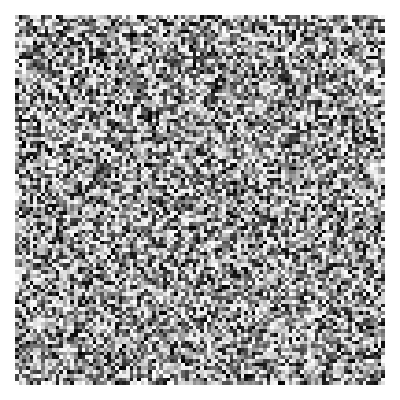
\includegraphics[width=.4\linewidth]{Images/gaussian_noise}
	}\qquad
	\subfloat[Perlin noise]{%
	\label{fig:perlin_noise}%
	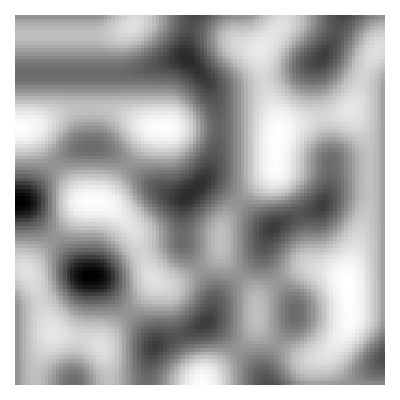
\includegraphics[width=.4\linewidth]{Images/perlin_noise}
	}
	\caption[Difference between noise patterns]{Difference between noise patterns.}
	\label{fig:noise_differences}
\end{figure}

\begin{figure}
	\centering
	\subfloat[Frequency 2]{%
	\label{fig:perlin_noise_2}%
	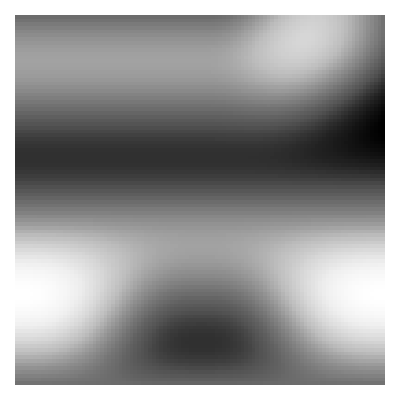
\includegraphics[width=.3\linewidth]{Images/perlin_noise_2}
	}\quad
	\subfloat[Frequency 5]{%
	\label{fig:perlin_noise_5}%
	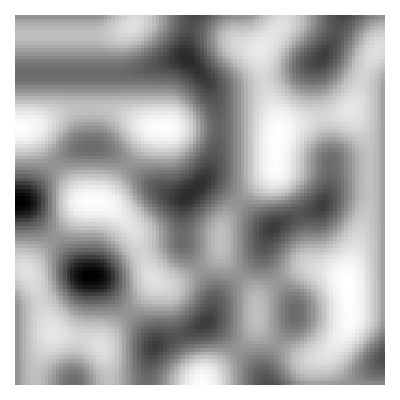
\includegraphics[width=.3\linewidth]{Images/perlin_noise}
	}\quad
	\subfloat[Frequency 20]{%
	\label{fig:perlin_noise_20}%
	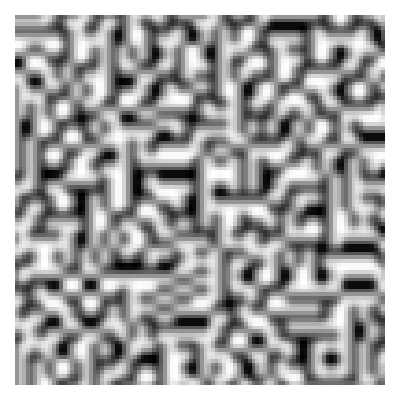
\includegraphics[width=.3\linewidth]{Images/perlin_noise_20}
	}
	\caption[Influence of frequency on Perlin noise]{Influence of frequency on Perlin noise patterns.}
	\label{fig:perlin_noise_frequencies}
\end{figure}

The second improvement is to use a regional mask. The original \gls{ba} applies a perturbation to the images as a whole. Every pixel will be perturbed with the same magnitude. This magnitude can be altered on a per-pixel basis when using a mask. Pixels that are further away from the target image will receive a larger perturbation than pixels that are already close to the corresponding pixel in the target. The mask $m$ is constructed according to equation \ref{eq:mask} based on the original image $x_{orig}$ and the adversarial image $x_{adv}$. It is then pixel-wise applied to the sampled perturbation in equation \ref{eq:mask_app}. The masked perturbation is normalized afterwards.\\ 

\begin{align}
m &= | x_{adv} - x_{orig}| \label{eq:mask}\\
\eta_{k} &= m \odot \eta_k; \eta_k = \frac{\eta_k}{\| \eta_k \|} \label{eq:mask_app}
\end{align}

This technique improves efficiency since the search space is significantly reduced. It is also possible to engineer masks for specific examples in order to incorporate other knowledge in the attack.\\

The final improvement is based on the idea of transfer attacks. A surrogate model is trained and will be used to calculate adversarial gradients. These gradients will then be used to bias the sampling direction for the orthogonal step. If the surrogate model does not closely resemble the defender, then the gradients will only hamper the speed of convergence of the attack instead of causing the attack to fail.

\begin{figure}
\centering
\tikzset{every picture/.style={line width=0.75pt}} %set default line width to 0.75pt        
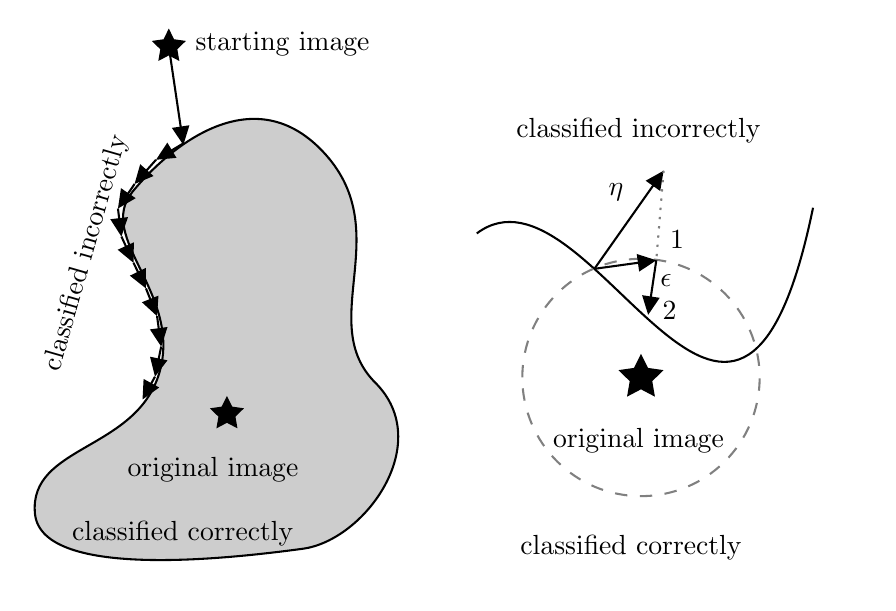
\begin{tikzpicture}[x=0.75pt,y=0.75pt,yscale=-1,xscale=1]
%uncomment if require: \path (0,300); %set diagram left start at 0, and has height of 300

%Shape: Polygon Curved [id:ds5185908380685693] 
\draw  [fill={rgb, 255:red, 155; green, 155; blue, 155 }  ,fill opacity=0.5 ] (77.12,91.56) .. controls (95.12,69.56) and (136.12,35.56) .. (170.12,73.56) .. controls (204.12,111.56) and (165.12,154.56) .. (194.12,183.56) .. controls (223.12,212.56) and (189.12,259.56) .. (159.12,263.56) .. controls (129.12,267.56) and (33.12,279.56) .. (30.12,246.56) .. controls (27.12,213.56) and (79.12,216.56) .. (90.12,178.56) .. controls (101.12,140.56) and (59.12,113.56) .. (77.12,91.56) -- cycle ;
%Shape: Star [id:dp7170747564600322] 
\draw  [fill={rgb, 255:red, 0; green, 0; blue, 0 }  ,fill opacity=1 ] (122.62,191.06) -- (124.83,195.53) -- (129.76,196.24) -- (126.19,199.72) -- (127.03,204.63) -- (122.62,202.31) -- (118.22,204.63) -- (119.06,199.72) -- (115.49,196.24) -- (120.42,195.53) -- cycle ;
%Shape: Star [id:dp10477759386916752] 
\draw  [fill={rgb, 255:red, 0; green, 0; blue, 0 }  ,fill opacity=1 ] (94.62,14.06) -- (96.83,18.53) -- (101.76,19.24) -- (98.19,22.72) -- (99.03,27.63) -- (94.62,25.31) -- (90.22,27.63) -- (91.06,22.72) -- (87.49,19.24) -- (92.42,18.53) -- cycle ;
%Straight Lines [id:da2531323347021954] 
\draw    (94.62,21.56) -- (101.19,66.01) ;
\draw [shift={(101.62,68.98)}, rotate = 261.6] [fill={rgb, 255:red, 0; green, 0; blue, 0 }  ][line width=0.08]  [draw opacity=0] (8.93,-4.29) -- (0,0) -- (8.93,4.29) -- cycle    ;
%Straight Lines [id:da6594852147606747] 
\draw    (101.79,68.14) -- (91.03,74.6) ;
\draw [shift={(88.46,76.14)}, rotate = 329.04] [fill={rgb, 255:red, 0; green, 0; blue, 0 }  ][line width=0.08]  [draw opacity=0] (8.93,-4.29) -- (0,0) -- (8.93,4.29) -- cycle    ;
%Straight Lines [id:da6002841525279263] 
\draw    (88.46,76.14) -- (80.11,85.56) ;
\draw [shift={(78.12,87.81)}, rotate = 311.53] [fill={rgb, 255:red, 0; green, 0; blue, 0 }  ][line width=0.08]  [draw opacity=0] (8.93,-4.29) -- (0,0) -- (8.93,4.29) -- cycle    ;
%Straight Lines [id:da9148455444041863] 
\draw    (78.12,87.81) -- (71.8,97.16) ;
\draw [shift={(70.12,99.64)}, rotate = 304.06] [fill={rgb, 255:red, 0; green, 0; blue, 0 }  ][line width=0.08]  [draw opacity=0] (8.93,-4.29) -- (0,0) -- (8.93,4.29) -- cycle    ;
%Straight Lines [id:da47669503735159546] 
\draw    (70.12,99.64) -- (71.42,110.17) ;
\draw [shift={(71.79,113.14)}, rotate = 262.96] [fill={rgb, 255:red, 0; green, 0; blue, 0 }  ][line width=0.08]  [draw opacity=0] (8.93,-4.29) -- (0,0) -- (8.93,4.29) -- cycle    ;
%Straight Lines [id:da26104674623686774] 
\draw    (71.79,113.14) -- (76.37,123.08) ;
\draw [shift={(77.62,125.81)}, rotate = 245.27] [fill={rgb, 255:red, 0; green, 0; blue, 0 }  ][line width=0.08]  [draw opacity=0] (8.93,-4.29) -- (0,0) -- (8.93,4.29) -- cycle    ;
%Straight Lines [id:da9792015265988265] 
\draw    (77.62,125.81) -- (82.31,135.45) ;
\draw [shift={(83.62,138.14)}, rotate = 244.06] [fill={rgb, 255:red, 0; green, 0; blue, 0 }  ][line width=0.08]  [draw opacity=0] (8.93,-4.29) -- (0,0) -- (8.93,4.29) -- cycle    ;
%Straight Lines [id:da8018833944649997] 
\draw    (83.62,138.14) -- (87.84,148.69) ;
\draw [shift={(88.96,151.48)}, rotate = 248.2] [fill={rgb, 255:red, 0; green, 0; blue, 0 }  ][line width=0.08]  [draw opacity=0] (8.93,-4.29) -- (0,0) -- (8.93,4.29) -- cycle    ;
%Straight Lines [id:da7469050329272713] 
\draw    (88.96,151.48) -- (90.55,163.17) ;
\draw [shift={(90.96,166.14)}, rotate = 262.23] [fill={rgb, 255:red, 0; green, 0; blue, 0 }  ][line width=0.08]  [draw opacity=0] (8.93,-4.29) -- (0,0) -- (8.93,4.29) -- cycle    ;
%Straight Lines [id:da36931886382540347] 
\draw    (90.96,166.14) -- (88.57,177.7) ;
\draw [shift={(87.96,180.64)}, rotate = 281.69] [fill={rgb, 255:red, 0; green, 0; blue, 0 }  ][line width=0.08]  [draw opacity=0] (8.93,-4.29) -- (0,0) -- (8.93,4.29) -- cycle    ;
%Straight Lines [id:da3125285737899821] 
\draw    (87.96,180.64) -- (83.39,189.01) ;
\draw [shift={(81.96,191.64)}, rotate = 298.61] [fill={rgb, 255:red, 0; green, 0; blue, 0 }  ][line width=0.08]  [draw opacity=0] (8.93,-4.29) -- (0,0) -- (8.93,4.29) -- cycle    ;

%Curve Lines [id:da7332610230112269] 
\draw    (243,111.62) .. controls (297.92,70.43) and (367.93,279.11) .. (405,99.26) ;
%Shape: Star [id:dp6998768571531213] 
\draw  [fill={rgb, 255:red, 0; green, 0; blue, 0 }  ,fill opacity=1 ] (322.11,170.74) -- (325.14,176.87) -- (331.9,177.85) -- (327.01,182.62) -- (328.16,189.36) -- (322.11,186.18) -- (316.06,189.36) -- (317.22,182.62) -- (312.32,177.85) -- (319.09,176.87) -- cycle ;
%Straight Lines [id:da9467918607674688] 
\draw    (299.68,128.68) -- (331.29,83.87) ;
\draw [shift={(333.02,81.42)}, rotate = 125.2] [fill={rgb, 255:red, 0; green, 0; blue, 0 }  ][line width=0.08]  [draw opacity=0] (8.93,-4.29) -- (0,0) -- (8.93,4.29) -- cycle    ;
%Shape: Ellipse [id:dp07084957668985581] 
\draw  [color={rgb, 255:red, 128; green, 128; blue, 128 }  ,draw opacity=1 ][dash pattern={on 4.5pt off 4.5pt}] (264.94,181.03) .. controls (264.94,149.46) and (290.54,123.86) .. (322.11,123.86) .. controls (353.69,123.86) and (379.28,149.46) .. (379.28,181.03) .. controls (379.28,212.61) and (353.69,238.2) .. (322.11,238.2) .. controls (290.54,238.2) and (264.94,212.61) .. (264.94,181.03) -- cycle ;
%Straight Lines [id:da7547924674466151] 
\draw    (299.68,128.68) -- (326.52,124.97) ;
\draw [shift={(329.49,124.56)}, rotate = 172.13] [fill={rgb, 255:red, 0; green, 0; blue, 0 }  ][line width=0.08]  [draw opacity=0] (8.93,-4.29) -- (0,0) -- (8.93,4.29) -- cycle    ;
%Straight Lines [id:da7777022216727221] 
\draw    (329.49,124.56) -- (326.01,147.88) ;
\draw [shift={(325.57,150.85)}, rotate = 278.49] [fill={rgb, 255:red, 0; green, 0; blue, 0 }  ][line width=0.08]  [draw opacity=0] (8.93,-4.29) -- (0,0) -- (8.93,4.29) -- cycle    ;
%Straight Lines [id:da931484330606797] 
\draw [color={rgb, 255:red, 128; green, 128; blue, 128 }  ,draw opacity=1 ] [dash pattern={on 0.84pt off 2.51pt}]  (333.02,81.42) -- (329.49,124.56) ;


% Text Node
\draw (328.21,263) node   [align=left] {\begin{minipage}[lt]{96.27pt}\setlength\topsep{0pt}
classified correctly
\end{minipage}};
% Text Node
\draw (326.21,62) node   [align=left] {\begin{minipage}[lt]{96.27pt}\setlength\topsep{0pt}
classified incorrectly
\end{minipage}};
% Text Node
\draw (325.12,211.56) node   [align=left] {\begin{minipage}[lt]{68pt}\setlength\topsep{0pt}
original image
\end{minipage}};
% Text Node
\draw (112.21,256.14) node   [align=left] {\begin{minipage}[lt]{96.27pt}\setlength\topsep{0pt}
classified correctly
\end{minipage}};
% Text Node
\draw (106,13) node [anchor=north west][inner sep=0.75pt]   [align=left] {starting image};
% Text Node
\draw (56.21,116) node  [rotate=-286.01] [align=left] {\begin{minipage}[lt]{96.27pt}\setlength\topsep{0pt}
classified incorrectly
\end{minipage}};
% Text Node
\draw (120.12,225.56) node   [align=left] {\begin{minipage}[lt]{68pt}\setlength\topsep{0pt}
original image
\end{minipage}};
% Text Node
\draw (381.43,114.71) node   [align=left] {\begin{minipage}[lt]{68pt}\setlength\topsep{0pt}
1
\end{minipage}};
% Text Node
\draw (377.9,148.85) node   [align=left] {\begin{minipage}[lt]{68pt}\setlength\topsep{0pt}
2
\end{minipage}};
% Text Node
\draw (330,130) node [anchor=north west][inner sep=0.75pt]   [align=left] {$\displaystyle \epsilon $};
% Text Node
\draw (305,86) node [anchor=north west][inner sep=0.75pt]   [align=left] {$\displaystyle \eta $};


\end{tikzpicture}
\caption[Intuition of the Boundary Attack]{Intuition behind the Boundary Attack. On the left the path of the attack is shown. The first step is a projection onto the boundary, afterwards it follows the decision boundary of the class of the original image. Each arrow represents one iteration of the attack. On the right, the two different steps of each iteration can be seen. In the first step, a random direction is sampled and projected onto a sphere around the original image. The second step is to take a step towards the original image from this new position. Image inspired by \cite{boundary_attack}.}
\label{fig:boundary_attack_intuition}
\end{figure}

\section{HopSkipJumpAttack}
\gls{hsja} \cite{hsja}, like \gls{ba}, is a decision-based adversarial attack that starts from an adversarial input. The initial input is obtained in an identical manner as in \gls{ba}. \gls{hsja} is an iterative algorithm that consists of three steps.\\

The first step is a projection onto the decision boundary of the model under attack. This projection is carried out using a binary search. The second step is to estimate the direction of the gradient at the boundary. Different directions are sampled from a uniform distribution over a $d$-dimensional sphere, where $d$ is the input dimension. This random direction is added to the boundary point, generating a new query for the model. The results of these queries are combined to a gradient estimation~$\widetilde{\nabla S}$ using the Monte Carlo estimate of equation \ref{eq:monte_carlo_estimate}. In this equation $u_b$ are the random directions and $x_t$ is the boundary position. $B$ is the number of random directions that needs to be sampled. This number increases based on the current iteration of the attack to reduce the variance of the estimate. The function~$\phi_{x^*}$ returns 1 if the new position is adversarial and -1 if it is not adversarial. $\delta$ is a positive parameter determining the size of the $d$-dimensional sphere.

\begin{equation}\label{eq:monte_carlo_estimate}
\widetilde{\nabla S}(x_t,\delta) := \frac{1}{B} \sum_{b=1}^{B}\phi_{x^*}(x_t + \delta u_b)u_b
\end{equation}

Once the gradient has been estimated, the third and final operation is to take a step along this gradient. The step size is determined using a geometric progression scheme. These steps are iteratively repeated until the pre-set stopping criterion is met. Figure \ref{fig:hsja_intuition} represents the intuition behind \gls{hsja} in a graphical manner.\\

\gls{hsja} eclipses \gls{ba} and \gls{bba} both on median distance against queries and attack success rates using a limited amount of queries. The untargeted version of \gls{hsja} is able to compete with white box attacks on the ImageNet dataset \cite{imagenet}. It also performs similar or superior to white box attacks such as the C\&W attack \cite{cw_attack} when evaluated against defensive mechanisms such as defensive distillation \cite{defensive_distillation}, region-based classification \cite{region-based_classification} and adversarial training \cite{FGSM}.


\begin{figure}
\centering


\tikzset{every picture/.style={line width=0.75pt}} %set default line width to 0.75pt        

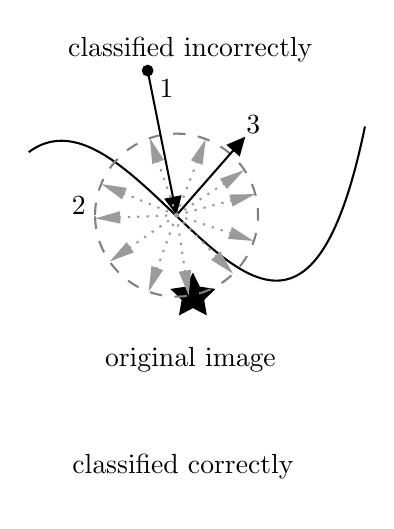
\begin{tikzpicture}[x=0.75pt,y=0.75pt,yscale=-1,xscale=1]
%uncomment if require: \path (0,300); %set diagram left start at 0, and has height of 300

%Curve Lines [id:da9704742483773781] 
\draw    (243,111.62) .. controls (297.92,70.43) and (367.93,279.11) .. (405,99.26) ;
%Shape: Star [id:dp26832364802919195] 
\draw  [fill={rgb, 255:red, 0; green, 0; blue, 0 }  ,fill opacity=1 ] (322.11,170.74) -- (325.14,176.87) -- (331.9,177.85) -- (327.01,182.62) -- (328.16,189.36) -- (322.11,186.18) -- (316.06,189.36) -- (317.22,182.62) -- (312.32,177.85) -- (319.09,176.87) -- cycle ;
%Shape: Ellipse [id:dp9511930412387599] 
\draw  [color={rgb, 255:red, 128; green, 128; blue, 128 }  ,draw opacity=1 ][dash pattern={on 4.5pt off 4.5pt}] (274.97,141.94) .. controls (274.97,120.26) and (292.54,102.69) .. (314.22,102.69) .. controls (335.9,102.69) and (353.48,120.26) .. (353.48,141.94) .. controls (353.48,163.63) and (335.9,181.2) .. (314.22,181.2) .. controls (292.54,181.2) and (274.97,163.63) .. (274.97,141.94) -- cycle ;
%Shape: Circle [id:dp5681517768642557] 
\draw  [fill={rgb, 255:red, 0; green, 0; blue, 0 }  ,fill opacity=1 ] (298,72.3) .. controls (298,71.03) and (299.03,70) .. (300.3,70) .. controls (301.57,70) and (302.6,71.03) .. (302.6,72.3) .. controls (302.6,73.57) and (301.57,74.6) .. (300.3,74.6) .. controls (299.03,74.6) and (298,73.57) .. (298,72.3) -- cycle ;
%Straight Lines [id:da06387380835189371] 
\draw    (300.3,72.3) -- (313.63,139) ;
\draw [shift={(314.22,141.94)}, rotate = 258.7] [fill={rgb, 255:red, 0; green, 0; blue, 0 }  ][line width=0.08]  [draw opacity=0] (8.93,-4.29) -- (0,0) -- (8.93,4.29) -- cycle    ;
%Straight Lines [id:da5011613685801404] 
\draw [color={rgb, 255:red, 155; green, 155; blue, 155 }  ,draw opacity=1 ][line width=0.75]  [dash pattern={on 0.84pt off 2.51pt}]  (314.22,141.94) -- (279.9,127.76) ;
\draw [shift={(278.05,127)}, rotate = 22.45] [fill={rgb, 255:red, 155; green, 155; blue, 155 }  ,fill opacity=1 ][line width=0.08]  [draw opacity=0] (12,-3) -- (0,0) -- (12,3) -- cycle    ;
%Shape: Boxed Line [id:dp5969211465757109] 
\draw [color={rgb, 255:red, 155; green, 155; blue, 155 }  ,draw opacity=1 ][line width=0.75]  [dash pattern={on 0.84pt off 2.51pt}]  (314.22,141.94) -- (327.54,107.28) ;
\draw [shift={(328.26,105.41)}, rotate = 111.02] [fill={rgb, 255:red, 155; green, 155; blue, 155 }  ,fill opacity=1 ][line width=0.08]  [draw opacity=0] (12,-3) -- (0,0) -- (12,3) -- cycle    ;
%Shape: Boxed Line [id:dp06580944891073615] 
\draw [color={rgb, 255:red, 155; green, 155; blue, 155 }  ,draw opacity=1 ][line width=0.75]  [dash pattern={on 0.84pt off 2.51pt}]  (314.22,141.94) -- (350.1,132.34) ;
\draw [shift={(352.03,131.82)}, rotate = 165.01] [fill={rgb, 255:red, 155; green, 155; blue, 155 }  ,fill opacity=1 ][line width=0.08]  [draw opacity=0] (12,-3) -- (0,0) -- (12,3) -- cycle    ;
%Shape: Boxed Line [id:dp5760742560965917] 
\draw [color={rgb, 255:red, 155; green, 155; blue, 155 }  ,draw opacity=1 ][line width=0.75]  [dash pattern={on 0.84pt off 2.51pt}]  (314.22,141.94) -- (340.03,168.65) ;
\draw [shift={(341.42,170.09)}, rotate = 225.98] [fill={rgb, 255:red, 155; green, 155; blue, 155 }  ,fill opacity=1 ][line width=0.08]  [draw opacity=0] (12,-3) -- (0,0) -- (12,3) -- cycle    ;
%Shape: Boxed Line [id:dp6962455418332032] 
\draw [color={rgb, 255:red, 155; green, 155; blue, 155 }  ,draw opacity=1 ][line width=0.75]  [dash pattern={on 0.84pt off 2.51pt}]  (314.22,141.94) -- (283.71,163.13) ;
\draw [shift={(282.07,164.27)}, rotate = 325.23] [fill={rgb, 255:red, 155; green, 155; blue, 155 }  ,fill opacity=1 ][line width=0.08]  [draw opacity=0] (12,-3) -- (0,0) -- (12,3) -- cycle    ;
%Straight Lines [id:da09211424476397356] 
\draw    (314.22,141.94) -- (345.36,106.42) ;
\draw [shift={(347.33,104.17)}, rotate = 131.23] [fill={rgb, 255:red, 0; green, 0; blue, 0 }  ][line width=0.08]  [draw opacity=0] (8.93,-4.29) -- (0,0) -- (8.93,4.29) -- cycle    ;
%Shape: Boxed Line [id:dp11391160549760482] 
\draw [color={rgb, 255:red, 155; green, 155; blue, 155 }  ,draw opacity=1 ][line width=0.75]  [dash pattern={on 0.84pt off 2.51pt}]  (314.22,141.94) -- (349.44,153.74) ;
\draw [shift={(351.34,154.37)}, rotate = 198.52] [fill={rgb, 255:red, 155; green, 155; blue, 155 }  ,fill opacity=1 ][line width=0.08]  [draw opacity=0] (12,-3) -- (0,0) -- (12,3) -- cycle    ;
%Shape: Boxed Line [id:dp7901030813069994] 
\draw [color={rgb, 255:red, 155; green, 155; blue, 155 }  ,draw opacity=1 ][line width=0.75]  [dash pattern={on 0.84pt off 2.51pt}]  (314.22,141.94) -- (302.05,106.86) ;
\draw [shift={(301.39,104.97)}, rotate = 70.87] [fill={rgb, 255:red, 155; green, 155; blue, 155 }  ,fill opacity=1 ][line width=0.08]  [draw opacity=0] (12,-3) -- (0,0) -- (12,3) -- cycle    ;
%Shape: Boxed Line [id:dp12912601709580973] 
\draw [color={rgb, 255:red, 155; green, 155; blue, 155 }  ,draw opacity=1 ][line width=0.75]  [dash pattern={on 0.84pt off 2.51pt}]  (314.22,141.94) -- (319.79,178.66) ;
\draw [shift={(320.09,180.64)}, rotate = 261.38] [fill={rgb, 255:red, 155; green, 155; blue, 155 }  ,fill opacity=1 ][line width=0.08]  [draw opacity=0] (12,-3) -- (0,0) -- (12,3) -- cycle    ;
%Shape: Boxed Line [id:dp15440737606551624] 
\draw [color={rgb, 255:red, 155; green, 155; blue, 155 }  ,draw opacity=1 ][line width=0.75]  [dash pattern={on 0.84pt off 2.51pt}]  (314.22,141.94) -- (301.49,176.83) ;
\draw [shift={(300.81,178.71)}, rotate = 290.05] [fill={rgb, 255:red, 155; green, 155; blue, 155 }  ,fill opacity=1 ][line width=0.08]  [draw opacity=0] (12,-3) -- (0,0) -- (12,3) -- cycle    ;
%Shape: Boxed Line [id:dp47011579703760575] 
\draw [color={rgb, 255:red, 155; green, 155; blue, 155 }  ,draw opacity=1 ][line width=0.75]  [dash pattern={on 0.84pt off 2.51pt}]  (314.22,141.94) -- (277.11,143.45) ;
\draw [shift={(275.11,143.53)}, rotate = 357.68] [fill={rgb, 255:red, 155; green, 155; blue, 155 }  ,fill opacity=1 ][line width=0.08]  [draw opacity=0] (12,-3) -- (0,0) -- (12,3) -- cycle    ;
%Shape: Boxed Line [id:dp3426945663084944] 
\draw [color={rgb, 255:red, 155; green, 155; blue, 155 }  ,draw opacity=1 ][line width=0.75]  [dash pattern={on 0.84pt off 2.51pt}]  (314.22,141.94) -- (345.13,121.35) ;
\draw [shift={(346.79,120.24)}, rotate = 146.33] [fill={rgb, 255:red, 155; green, 155; blue, 155 }  ,fill opacity=1 ][line width=0.08]  [draw opacity=0] (12,-3) -- (0,0) -- (12,3) -- cycle    ;

% Text Node
\draw (328.21,263) node   [align=left] {\begin{minipage}[lt]{96.27pt}\setlength\topsep{0pt}
classified correctly
\end{minipage}};
% Text Node
\draw (326.21,62) node   [align=left] {\begin{minipage}[lt]{96.27pt}\setlength\topsep{0pt}
classified incorrectly
\end{minipage}};
% Text Node
\draw (325.12,211.56) node   [align=left] {\begin{minipage}[lt]{68pt}\setlength\topsep{0pt}
original image
\end{minipage}};
% Text Node
\draw (304.6,75.3) node [anchor=north west][inner sep=0.75pt]   [align=left] {1};
% Text Node
\draw (262.33,131.33) node [anchor=north west][inner sep=0.75pt]   [align=left] {2};
% Text Node
\draw (346.33,92.67) node [anchor=north west][inner sep=0.75pt]   [align=left] {3};
\end{tikzpicture}
\caption[Intuition of the HopSkipJumpAttack]{Intuition behind the HopSkipJumpAttack. Each iteration consists of three steps. The first step is a projection onto the boundary. The second step is the estimation of the gradient at this point. This is done by sampling directions from a uniform distribution and querying the model under attack from this new position (grey arrows). The results are combined via the Monte Carlo estimate. The third and final step is to take a step along the estimated gradient. Image inspired by \cite{hsja}.}
\label{fig:hsja_intuition}
\end{figure}

\section{Stateful defense}\label{sec:stateful_detection}
The defensive schemes discussed in section \ref{sec:adversarial_defenses} all operate on the query level. They try to detect and flag possible attacks based on a single query without taking other context into account. The stateful detection mechanism by Chen, Carlini and Wagner \cite{chen_stateful_2019} is different in this aspect. As the name suggests, it holds state of previously submitted queries. It is similar to the defenses that use proximity measurements, but the measurement is between queries instead of between the query and training data.\\

All queries submitted to the model equipped with a stateful detection mechanism are stored in a history buffer. Each user of the model has a distinct history buffer, where its queries are stored. These buffers can be bounded by time or number of queries depending on the resources available and the use case of the model. Each time a query is submitted to the model, the average distance to its $k$ nearest neighbors is calculated and if this distance is lower than a certain threshold, then the user gets flagged by the mechanism. Appropriate actions such as banning the account can be taken.\\

The distance metric is not calculated in input space. Each query is encoded by a deep similarity encoder \cite{deep_similarity_encoder} to an encoded space, typically of a lower dimension. In this encoded space, images which represent perceptually similar objects are clustered together. The advantage of the encoded space is twofold. Firstly, the dimension of the encoded space is smaller than the dimension of the input space. Therefore less space is needed to store the history buffers. Secondly, simpler distance metrics such as $L_2$-distance in input space can easily be evaded by an attacker. For example the $L_2$-distance can be significantly increased by simply rotating or shifting the input image.\\

The parameter $k$, the number of neighbors to consider is picked as follows. As the training data of the model consists of only benign queries, no attacks should be flagged when feeding the stateful detection mechanism with this data. To allow for some more leniency, a false positive rate of 0.1\% is still acceptable. For each value of $k$, a different threshold will be required to maintain the selected false positive rate. Larger values have the benefit of larger thresholds causing the defense to be more resilient, since attackers' images need to be more diverse. But $k$ is also the number of queries needed before an attack can be flagged. Therefore too large values for $k$ are disadvantageous. Smaller values also reduce computational cost. Chen, Carlini and Wagner set the value of $k$ to 50 for the CIFAR-10  dataset \cite{cifar}, since the thresholds increased sharply up to this value. Other datasets might require different values for $k$.

\section{PSO and distributed attacks}\label{sec:pso_and_distributed_attacks}
There have been several attempts to craft adversarial examples using an \gls{ea}. Previous attempts tried to reduce the number of queries needed to create a successful adversarial example by utilizing \glspl{ea} \cite{genattack,dong2019efficient,mosli2019they,audio_pso,distributed_pso_attack,suryanto2020}. \\

GenAttack \cite{genattack} and the similar efficient attack by Dong et al. \cite{dong2019efficient} use genetic algorithms in order to minimize the number of queries to the model. Both algorithms reduce the dimension of the search space to improve the efficiency of the attack. Once a promising perturbation is found in this lower dimensional space, it is upscaled using a bilinear transformation. By reducing the search space, the number of individuals in the genetic algorithm can be lowered, which in turn lowers the total amount of queries. GenAttack also uses annealing schemes to adaptively scale the parameters of the algorithm. This allows it to escape local optima and improve the adversarial example further. \\

AdversarialPSO \cite{mosli2019they} and the similar attack from \cite{audio_pso} use \gls{pso} as optimization routine on images and audio fragments respectively. Each particle represents a possible adversarial example. Both attacks use the standard rules of \gls{pso} as specified by \cite{pso} improved with a linearly decaying inertia weight \cite{inertia_weight}. The former attack also uses a constriction factor to avoid premature convergence \cite{constriction_factor}. While the latter solves this problem by generating new particles using a genetic algorithm when premature convergence is detected. Both algorithms rely on confidence scores to assign fitness values to certain positions in the search space. \gls{pso}-\gls{bba} \cite{distributed_pso_attack}, is similar to AdversarialPSO, but only relies on distances to determine fitness values. This attack can therefore also be used in decision-based settings instead of solely in score-based settings.\\

The idea behind the multi-group \gls{pso} attack \cite{suryanto2020} is to use multiple \gls{pso} swarms to escape local optima. The intuition behind it is inspired by the \gls{ddos} attack \cite{ddos}. The swarm is split into multiple smaller groups and each group is placed on a single node. The groups perform the standard \gls{pso} algorithm. The best position over all groups is communicated using a dedicated server. Each group submits its queries from its own node, tricking the defensive mechanism into thinking that multiple users are submitting queries. The authors state that this will ultimately result in less detections, but they have not evaluated this against a defensive scheme.\\
